\documentclass{article}
\usepackage[]{url}
\usepackage{graphicx}
\usepackage{hyperref}
\usepackage{mathtools}
\usepackage{tikz}
\usepackage{subcaption}
\usepackage{float}

\begin{document}
\title{Collective motion of squirmers in confined environments}
\author{Roth Robin\\
\\
Supervisors: Van Landeghem Céline, Giraldi Laetitia,\\ Agathe Chouippe}
\date{May, 2024}
\maketitle

\tableofcontents

\section{Introduction}
This internship is the continuation of a project realised during the year. The main goal of the project was
to develop numerical methods for driving micro-robots composed of magnetic heads and flexible tails imitating spermatozoa, reffered to as squirmers.\\
A python code has been implemented during the project, it simulates the behaviors of two interacting squirmers by computing 
the forces and torques present.\\
\section{Context}
The collective behavior of active particles is well studied in the literature. 
The Vicsek model is frequently used to model these active particles. 
The aim of this internship is to perform a similar study considering squirmers, 
in various confined domains and to compare the collective motion of the squirmers with that of the active particles using the Vicsek model. 
The motion of the squirmers is simulated using two different models: a continuous model that approximates hydrodynamic and 
steric forces, and a full model using the finite element library Feel++.

\section{Objectives}
The main goal is to model the dynamics of a group of squirmers within confined environments and to
 study the parameter that affect the alignement of the squirmers.

\section{Vicsek}
\subsection{Model}
\begin{center}
    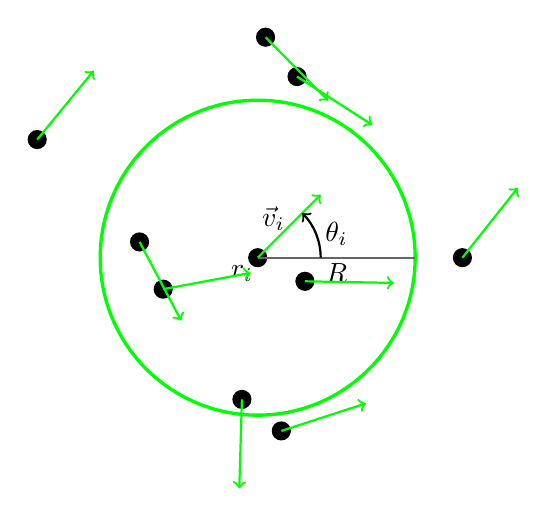
\begin{tikzpicture}
        \draw[color=green, very thick](0,0) circle (2);
        \node at (-0.2,-0.2) {{$r_i$}};
        \filldraw[color=black, fill=black, very thick](0,0) circle(0.1);
        \filldraw[color=black, fill=black, very thick](-1.5,0.2) circle(0.1);
        \filldraw[color=black, fill=black, very thick](0.5,2.3) circle(0.1);
        \filldraw[color=black, fill=black, very thick](2.6,0) circle(0.1);
        \filldraw[color=black, fill=black, very thick](-0.2,-1.8) circle(0.1);
        \filldraw[color=black, fill=black, very thick](0.6,-0.3) circle(0.1);
        \filldraw[color=black, fill=black, very thick](-1.2,-0.4) circle(0.1);
        \filldraw[color=black, fill=black, very thick](-2.8,1.5) circle(0.1);
        \filldraw[color=black, fill=black, very thick](0.3,-2.2) circle(0.1);
        \filldraw[color=black, fill=black, very thick](0.1,2.8) circle(0.1);
        \draw[thick, -, color=black!60] (0,0) -- (2,0);
        \node at (1,-0.2) {{$R$}};
        %Length of the arrow
        \pgfmathsetmacro{\len}{sqrt(1.28)}

        %Draw arrows with random directions
        \foreach \x/\y in {-1.5/0.2, 0.5/2.3, 2.6/0, -0.2/-1.8, -1.2/-0.4, -2.8/1.5, 0.3/-2.2, 0.1/2.8} {
            \pgfmathsetmacro{\angle}{random()*360}
            \draw[thick, ->, color=green] (\x,\y) -- ++({\len*cos(\angle)},{\len*sin(\angle)});
        }
        \draw[thick, ->, color=green] (0,0) -- (0.8,0.8);
        \draw[thick, ->, color=green] (0.6, -0.3) -- ++ ({\len*cos(-1.04)},{\len*sin(-1.04)});
        \node [color=black] at (0.2,0.5) {{$\vec{v}_i$}};
        \draw[thick, ->, color=black] (0.8, 0) arc (0:45:0.8);
        \node at (1, 0.3) {{$\theta_i$}};
    \end{tikzpicture}
\end{center}

The Vicsek model consists of $N$ particles with $r_i(t)$ and $\theta_i(t)$ 
their positions and orientations.\\
All particles have the same velocity $v_0$ and radius.
The evolution of the orientation $\theta_i(t)$ at each time step $\nabla t$ is:
$$\theta_i(t + \nabla t) = \langle\theta_j(t)\rangle_{|r_i(t) - r_j(t)| < R} + \epsilon_i(t)$$
with
$$\langle\theta_j(t)\rangle = \arctan\left(\frac{\sin(\theta_j(t))}{\cos(\theta_j(t))}\right)$$
$R$ the range of interaction, $\langle\theta_j(t)\rangle_{|r_i(t) - r_j(t)| < R}$ the average 
orientation of the particles in the range $R$ of
 the $i$-the particle (including itself) at the time $t$ and $\epsilon_i(t)$ represents the noise, 
 it's a random number taken from a uniform probability distribution
over $\left(-\frac{\eta}{2}, \frac{\eta}{2}\right)$.\\
The parameter $\eta$ is the main tool that counteracts the alignment of the particles.\\
\\
The evolution of the position $r_i(t)$ at each time step $\nabla t$ is:
$$ r_i(t + \nabla t) = r_i(t) + v_0\nabla t \begin{pmatrix}
    \cos(\theta_i(t))\\
    \sin(\theta_i(t))
\end{pmatrix}$$
The velocity is described by $\vec{v}_i(t)$ which is defined by
$$\vec{v}_i(t) = v_0\begin{pmatrix}
    \cos\theta_i(t)\\
    \sin\theta_i(t)
\end{pmatrix}$$
The behavior of the particles are quantified by the polar order parameter $v_a$ which is calculated with:
$$v_a = \frac{1}{Nv_0}\left|\sum^{N}_{i=1}\vec{v}_i\right|$$

\subsection{Implementation}
The Vicsek model is implemented in the file \texttt{Code/vicsek.py} as a class 
for a square system with repulsive borders
\subsubsection*{Parameters}
\begin{itemize}
    \item $N$ the number of particles in the system
    \item $R$ the range of interaction of the particles
    \item $L$ the length of the system
    \item $v0$ the constant velocity of the particles
    \item $radius$ the radius of the particles
    \item $T$ the time of simulation
    \item $dt$ the time step between each iteration
    \item $noise$ the $\eta$ parameter, used to counteract the alignment of the particles
    \item $beta$ is a parameter which initializes the Squirmers but
    is not used
\end{itemize}
When called, the class initializes $N$ particles with random position and orientation within the square.
\subsubsection*{Methods}
\begin{itemize}
    \item \texttt{distance(p1, p2)} returns the distance between the two particles in argument
    \item \texttt{dist\_particles(particle)} returns a list of the distance between the particle in argument and all of the other ones
    \item \texttt{how\_many\_in\_square()} prints and returns the percentage of particles inside the square. It is
    used to test if the code contains errors.
    \item \texttt{ploar\_order\_parameter()} computes and returns $v_a$ the polar order parameter
    \item \texttt{ref\_border\_x(particle, boundary)} and \texttt{ref\_border\_y(particle, boundary)}
    simulates the reflective borders
    \item \texttt{vector\_x(p1, p2)} and \texttt{vector\_y(p1, p2)} returns respectively the vector in the x and y axis of the
    two particles in argument
    \item \texttt{average\_orient(particle)} returns the average orientation of the particles in a range $R$ of the particle in argument (including itself)
    \item \texttt{update\_orient()} computes the orientation $\theta_i(t + \nabla t)$ by using \texttt{average\_orient}
    \item \texttt{update\_position()} computes the position $r_i(t + \nabla t)$ and uses the reflective borders if necessary
    \item \texttt{loop\_time()} uses \texttt{update\_orientation()} and \texttt{update\_position()} for each time step $dt$
    \item \texttt{plot(ax)} plots the square and the particles in the ax
\end{itemize}

\newpage
\section{Squirmer model}
\begin{center}
   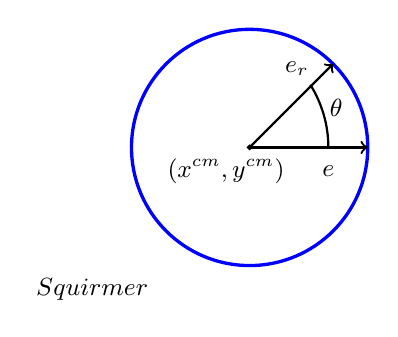
\begin{tikzpicture}
      \small
      
      \draw[color=blue, very thick](2.5,2.5) circle (1.5);
      
      \draw[color=black, very thick](2.5,2.5) circle (0.01);
      
      \node  at (2.5-0.3,2.5-0.3) {{$(x^{cm},y^{cm})$}};
      
      \node  at (0.5,0.7) {{$Squirmer$}};
      
      \draw[thick, ->] (2.5,2.5) -- (4,2.5);
      \node  at (3.5,2.2) {{$e$}};
   
      \pgfmathsetmacro{\xcoord}{2.5 + 1.5*cos(45)}
       \pgfmathsetmacro{\ycoord}{2.5 + 1.5*sin(45)}
       \draw[thick, ->] (2.5,2.5) -- (\xcoord,\ycoord);
      \node  at (3.1,3.5) {{$e_r$}}; 
      \draw[thick, -] (3.5,2.5) arc[start angle=0, end angle=32, radius=1.5];
      \node at (3.6,3) {${\theta}$}; 
      
         
      \end{tikzpicture}
    \end{center}
The time-independent velocity $u$ defined on the surface of the squirmer is given 
in polar coordinates by :

\begin{align*}
   \left\{\begin{array}{rcl}
      u_r(R,\theta) &=& 0 \\
      u_\theta(R,\theta) &=& B_1\mathrm{sin}(\theta)+B_2\mathrm{sin}(\theta)\mathrm{cos}(\theta)
   \end{array}\right.\;
\end{align*} \cite{Lauga}

By setting $\beta=\frac{B_2}{B_1}$, we have :
$$
u_\theta(R,\theta) = B_1(\mathrm{sin}(\theta) + \beta \mathrm{sin}(\theta)\mathrm{cos}(\theta)),
$$
where $\beta$ is the type of the squirmer :
$$\left\{
    \begin{array}{ll}
        \beta = 0 : \text{neutral swimmer}  \\
        \beta < 0 : \mathrm{pusher} \\
        \beta > 0 : \mathrm{puller} \\
    \end{array}
\right.$$
and $B_1$ describes the swimming velocity $v_0 = \frac{2 B_1}{3}$.
\\ Now let us put $u$ in cartesian coordinates :
\begin{align*}
    u &= \begin{pmatrix}
   u_x \\
   u_y
\end{pmatrix}
= \begin{pmatrix}
   \mathrm{cos}(\theta) & -\mathrm{sin}(\theta) \\
   \mathrm{sin}(\theta) & \mathrm{cos}(\theta)
\end{pmatrix}
\begin{pmatrix}
   u_r \\
   u_\theta
\end{pmatrix}, \\
&= B_1 (1 + \beta \mathrm{cos}(\theta))
\begin{pmatrix}
   -\mathrm{sin}^2(\theta) \\
   \mathrm{sin}(\theta)\mathrm{cos}(\theta)
\end{pmatrix}.
\end{align*}

We define $e_r$ the unit vector pointing from the center to the surface 
$$
e_r = \begin{pmatrix}
   \frac{x - x^{cm}}{r}  \\
   \frac{y - y^{cm}}{r} 
\end{pmatrix} = \begin{pmatrix}
   \mathrm{cos}(\theta) \\
   \mathrm{sin}(\theta)
\end{pmatrix}$$ 

and $e$ = 
$\begin{pmatrix}
   \mathrm{cos}(\phi) \\
   \mathrm{sin}(\phi) \end{pmatrix}$ the swimming direction of the squirmer. 
   
   By fixing $\phi$ = 0, one has $e$ = $\begin{pmatrix}
   1 \\
   0 \end{pmatrix}$ and one finds the following expression for the velocity field 
   in cartesian coordinates: 

\begin{align*}
u &= B_1 \left(1+\beta \mathrm{cos}(\theta) \right) \begin{pmatrix}
   -\mathrm{sin}^2(\theta) \\
   \mathrm{sin}(\theta)\mathrm{cos}(\theta)
\end{pmatrix},  \\
&= B_1 \left(1+\beta \mathrm{cos}(\theta) \right) \begin{pmatrix}
   \mathrm{cos}^2(\theta)-1 \\
   \mathrm{sin}(\theta)\mathrm{cos}(\theta)
\end{pmatrix}, \\
&= B_1 \left(1+\beta \begin{pmatrix}
   1 \\
   0 \end{pmatrix}\begin{pmatrix}
   \mathrm{cos}(\theta) \\
   \mathrm{sin}(\theta)
\end{pmatrix}\right) \left[ \left( \begin{pmatrix}
   1 \\
   0 \end{pmatrix}\begin{pmatrix}
   \mathrm{cos}(\theta) \\
   \mathrm{sin}(\theta)
\end{pmatrix}\right) \begin{pmatrix}
   \mathrm{cos}(\theta) \\
   \mathrm{sin}(\theta)
\end{pmatrix} - \begin{pmatrix}
   1 \\
   0 \end{pmatrix}\right], \\
&= B_1(1+\beta (e \cdot e_r)) [(e \cdot e_r)e_r - e]. 
\end{align*}

\vspace{0.5 cm}
Thus, $u$ in cartesian coordinates is given by :
\begin{equation*}
\boxed{u_r = B_1(1+\beta (e\cdot e_r)) [(e\cdot e_r)e_r - e].}
\end{equation*}


\section{Dynamics of two interacting squirmers}
\subsection{The evolution of the mass center $R_i$}
The evolution of the mass center $R_i$ = $(X_i, Y_i)$ of one squirmer $i$ in presence of 
another squirmer $j$ and rigid boundaries, is given by :
\begin{center}
$\boxed{\frac{dR_i}{dt}$ = $v_0 p_i -  \nabla_{R_{ij}} V_{ij} - \partial_{R_i} V_i + F^{hydro} + \sqrt{2D}\eta_i(t)}$
\end{center}
We have : \begin{itemize}
    \item $v_0$ the particle swimming velocity,
    \item $p_i$ = $(\mathrm{cos}(\theta),\mathrm{sin}(\theta))$ orientation,
    \item $F^{hydro}$ the lubrification forces given by Brumley\cite{Brumley},
    \item $V_{ij}$ and $V_i$, Weeks-Chandler-Andersen potential : repulsive steric force avoiding the overlapping of two squirmers or of one squirmer and a rigid boundary. The force is activated when the distance between two surfaces is small,
    \item $D$ the translational diffusivity
    \item $\eta_i$'s are independent noises. 
\end{itemize} 
\vspace{0,5cm}
$V_{ij}$ = $\frac{E_s}{6\pi\mu r}\left[\left(\frac{2r}{\lvert R_{ij}\rvert}\right)^{12} - \left(\frac{2r}{\lvert R_{ij}\rvert}\right)^6\right]$ and  $V_i$ = $\frac{E_s}{6\pi\mu r} \left[ \left( \frac{r}{\lvert R - R_i \rvert} \right)^{12} - \left( \frac{r}{\lvert R - R_i \rvert} \right) ^6 \right]$ 
\vspace{0,3cm}
\\With : \begin{itemize}
    \item $R_{ij}$ = $\sqrt{D_x^2+D_y^2}$, $\lvert R_{ij} \rvert$ the distance between the centers of two squirmers,
    \item $\lvert R - R_i\rvert$ the distance between the wall and the squirmer center,
    \item $E_s$ a positive constant,
    \item $r$ the radius of a squirmer,
    \item $\mu$ the dynamic viscosity.
\end{itemize}

\vspace{0,5cm}
We want to compute the steric force, given by $\nabla_{R_{ij}} V_{ij}$:

\begin{align*}
\frac{\partial V_{ij}}{\partial D_x} &= \frac{\partial}{\partial D_x}\frac{E_s}{6\pi\mu r}\left[\left(\frac{2r}{\lvert R_{ij}\rvert}\right)^{12} - \left(\frac{2r}{\lvert R_{ij}\rvert}\right)^6\right] \\
&= \frac{E_s}{6\pi\mu r} \left[\frac{\partial}{\partial D_x}\left(\frac{2r}{\lvert R_{ij}\rvert}\right)^{12} - \frac{\partial}{\partial D_x} \left(\frac{2r}{\lvert R_{ij}\rvert}\right)^6\right] \\
&= \frac{E_s}{6\pi\mu r} \left[ \frac{-12 D_x (2r)^{12}(R_{ij})^{10}}{(R_{ij})^{24}} - \frac{-6D_x(2r)^6(R_{ij})^4}{(R_{ij})^{12}}  \right] \\
&= \frac{-12 E_s}{2r6\pi\mu r} \left[ \frac{D_x (2r)^{13}}{(R_{ij})^{14}} - \frac{D_x (2r)^{7}}{2(R_{ij})^8}\right] \\
&= -\frac{E_s}{r^2\pi\mu} \frac{D_x}{R_{ij}} \left[ \frac{(2r)^{13}}{(R_{ij})^{13}} - \frac{(2r)^7}{2(R_{ij})^{7}}\right]
\end{align*}
Equivalently, we have : 
$\frac{\partial V_{ij}}{\partial D_y}$ = $-\frac{E_s}{r^2\pi\mu} \frac{D_y}{R_{ij}}\left[ \frac{(2r)^{13}}{(R_{ij})^{13}} - \frac{(2r)^7}{2(R_{ij})^7} \right]$
\\ We find : 
\begin{equation*}
    \boxed{\nabla_{R_{ij}} V_{ij} = 
    \begin{pmatrix}
        -\frac{E_s}{r^2\pi\mu} \frac{D_x}{R_{ij}}\left[ \frac{(2r)^{13}}{(R_{ij})^{13}} - \frac{(2r)^7}{2(R_{ij})^7} \right] \\
        -\frac{E_s}{r^2\pi\mu} \frac{D_y}{R_{ij}}\left[ \frac{(2r)^{13}}{(R_{ij})^{13}} - \frac{(2r)^7}{2(R_{ij})^7} \right]
    \end{pmatrix}}
\end{equation*}

\vspace{0,5cm}

In addition, we need to compute $\partial_{R_i} V_i$ to obtain the force applied between a squirmer and a rigid boundary.

\begin{align*}
    \frac{\partial V_i}{\partial X} &= \frac{\partial}{\partial X} \left( \frac{E_s}{6\pi\mu r} \left[ \left( \frac{r}{\lvert R - R_i \rvert} \right)^{12} - \left( \frac{r}{\lvert R - R_i \rvert} \right) ^6 \right] \right) \\
    &= \frac{\partial}{\partial X} \left( \frac{E_s}{6\pi\mu r} \left[ \left( \frac{r}{\sqrt{( X-X_{box})^2 + (Y-Y_{box})^2)}} \right)^{12} - \left( \frac{r}{\sqrt{( X-X_{box})^2 + (Y-Y_{box})^2)}} \right) ^6 \right] \right) \\
    &= \frac{E_s}{6\pi\mu r}\left[ 12(X_{box}-X)\frac{r^{12}}{\lvert R - R_i\rvert^{14}} - 6(X_{box}-X)\frac{r^6}{\lvert R-R_i\rvert^8} \right] \\
    &= -\frac{E_s (X-X_{box})}{\pi\mu r^2 \lvert R - R_i \rvert } \left[ 2 \left( \frac{r}{\lvert R-R_i\rvert} \right)^{13} - \left( \frac{r}{\lvert R-R_i\rvert}\right)^7 \right] 
\end{align*}
Equivalently, we have : $\frac{\partial V_i}{\partial Y}$ = $ - \frac{E_s (Y-Y_{box})}{\pi\mu r^2 \lvert R - R_i \rvert } \left[ 2 \left( \frac{r}{\lvert R-R_i\rvert} \right)^{13} - \left( \frac{r}{\lvert R-R_i\rvert}\right)^7 \right]$

We have : 
\begin{equation*}
    \boxed{\nabla_{R_i} V_i = \begin{pmatrix}
        -6 \frac{E_s (X-X_{box})}{\pi\mu r^2 \lvert R - R_i \rvert } \left[ 2 \left( \frac{r}{\lvert R-R_i\rvert} \right)^{13} - \left( \frac{r}{\lvert R-R_i\rvert}\right)^7 \right] \\
        -6 \frac{E_s (Y-Y_{box})}{\pi\mu r^2 \lvert R - R_i \rvert } \left[ 2 \left( \frac{r}{\lvert R-R_i\rvert} \right)^{13} - \left( \frac{r}{\lvert R-R_i\rvert}\right)^7 \right]
    \end{pmatrix}}
\end{equation*}

\begin{center}
   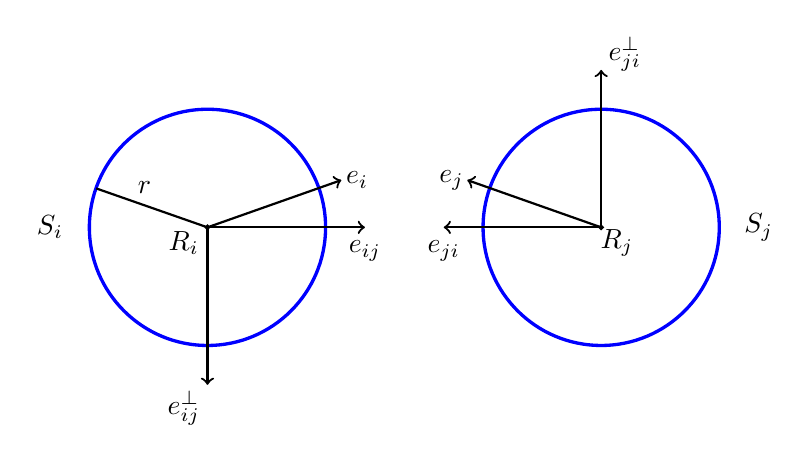
\begin{tikzpicture}
   
   \draw[color=blue, very thick](5,5) circle (1.5);
   \draw[color=blue, very thick](0,5) circle (1.5);
   
   \draw[color=black, very thick](0,5) circle (0.01);
   \draw[color=black, very thick](5,5) circle (0.01);
   
   \node  at (-0.3,5-0.2) {{$R_i$}};
   \node  at (5+0.2,5-0.2) {{$R_j$}};
   
   \node  at (-2,5) {{$S_i$}};
   \node  at (7,5) {{$S_j$}};
   
   \draw[thick, ->] (0,5) -- (1.7,5+0.6);
   \draw[thick, ->] (5,5) -- (5-1.7,5+0.6);
   
   \node  at (1.9,5+0.6) {{$e_i$}};
   \node  at (5-1.9,5+0.6) {{$e_j$}};
   
   \draw[thick] (0,5) -- ({-cos(45)*2}, {5+0.7*sin(45)});
   \node  at (-0.8,5+0.5) {{$r$}};
   
   \draw[thick, ->] (0,5) -- (2,5);
   \draw[thick, ->] (5,5) -- (3,5);
   
   \node  at (2,5-0.3) {{$e_{ij}$}};
   \node  at (3,5-0.3) {{$e_{ji}$}};
   
   \draw[thick, ->] (0,5) -- (0,3);
   \node  at (-0.3,3-0.3) {$e^{\perp}_{ij}$};
   
   
   \draw[thick, ->] (5,5) -- (5,7);
   \node  at (5+0.3,7+0.2) {$e^{\perp}_{ji}$};
   
   \end{tikzpicture}
   \end{center}
The figure shows the different vectors involved in the computations which will follow.
\\We define : 
\begin{itemize}
    \item $W_n(\mathrm{cos}(\theta))$ = $\frac{2}{n(n+1)}P_n'(\mathrm{cos}(\theta))$ \cite{Brumley}
    \item $P_n(\mathrm{cos}(\theta))$ the Legendre polynomials \cite{Wikipedia}
    \item $e_i.e_{ij} = \mathrm{cos}(\theta)$
    \item $e_i.e^{\perp}_{ij}$ = $\frac{(Y_{R_j} - Y_{R_i})\mathrm{cos}(\theta) - (X_{R_j} - X_{R_i})\mathrm{sin}(\theta)}{\lvert R_{ij} \rvert} $
\end{itemize}

The tangential lubrification forces acting on the two spheres can be calculated explicitly by :
\\ $F_z^{S_i}$ = $-9 \mu \pi r \frac{\lambda ^2}{(\lambda +1)^2} \sum_{n} \left[ B_n W_n(-e_i.e_{ij})e_i.e_{ij} + \frac{1}{2} B_n W_n'(-e_i.e_{ij})(e_i.e^{\perp}_{ij})^2 \right] (ln \epsilon + O(1))$ \cite{Brumley}

For $n$ = 1 : \begin{align*}
    W_1(\mathrm{-cos}(\theta)) &= \mathrm{sin}(\theta) \\
    W_1'(\mathrm{-cos}(\theta)) &= \mathrm{cos}(\theta) \\
    B_1 W_1(\mathrm{-cos}(\theta))e_i.e_{ij}+ \frac{1}{2} B_1  W_1'(\mathrm{-cos}(\theta)) (e_i.e^{\perp}_{ij})^2  &= B_1 \mathrm{sin}(\theta)e_i.e_{ij} + \frac{1}{2} B_1  \mathrm{cos}(\theta) (e_i.e^{\perp}_{ij})^2 \\
    &= B_1 \mathrm{sin}(\theta)\mathrm{cos}(\theta) + \frac{1}{2} B_1  \mathrm{cos}(\theta) (e_i.e^{\perp}_{ij})^2
\end{align*} 
For $n$ = 2 : \begin{align*}
    W_2(\mathrm{-cos}(\theta)) &= \mathrm{cos}(\theta)\mathrm{sin}(\theta) \\
    W_2'(\mathrm{-cos}(\theta)) &= 2\mathrm{cos}^2(\theta) - 1\\
    B_2 W_2(\mathrm{-cos}(\theta))e_i.e_{ij}+ \frac{1}{2} B_2  W_2'(\mathrm{-cos}(\theta)) (e_i.e_x)^2  &= B_2 \mathrm{sin}(\theta)\mathrm{cos}(\theta)e_i.e_{ij} + \frac{1}{2} B_2(2\mathrm{cos}^2(\theta) - 1) (e_i.e^{\perp}_{ij})^2 \\
    &= B_2 \mathrm{sin}(\theta)\mathrm{cos}^2(\theta) + \frac{1}{2} B_2(2\mathrm{cos}^2(\theta) - 1) (e_i.e^{\perp}_{ij})^2
\end{align*}  

So :
\begin{equation*}
\footnotesize
\boxed{
    F_z^{S_i} = -9 \mu \pi r \frac{\lambda ^2}{(\lambda +1)^2} \left[ B_1 \mathrm{sin}(\theta)\mathrm{cos}(\theta) + \frac{1}{2} B_1  \mathrm{cos}(\theta) (e_i.e^{\perp}_{ij})^2 +B_2 \mathrm{sin}(\theta)\mathrm{cos}^2(\theta) + \frac{1}{2} B_2(2\mathrm{cos}^2(\theta) - 1) (e_i.e^{\perp}_{ij})^2\right](ln \epsilon + O(1))}
\end{equation*}
\normalsize
\vspace{0.5cm}

The normal forces acting on the two spheres can be calculated explicitly by: \\
 $F_x^{S_i}$ = $-\frac{4}{5} \mu \pi r \frac{\lambda(\lambda +4)}{(\lambda +1)^2} \sum_{n} B_n W_n(e_i.e_{ij}) (ln \epsilon + O(1))$ \cite{Brumley}
\\ So :
\begin{equation*}
    \footnotesize
    \boxed{F_x^{S_i} = -\frac{4}{5} \mu \pi r \frac{\lambda(\lambda +4)}{(\lambda +1)^2} \left[ B_1\mathrm{sin}(\theta) +B_2\mathrm{cos}(\theta)\mathrm{sin}(\theta)\right] (ln \epsilon + O(1))}
\end{equation*}

The effect of a wall can be calculated by replacing one of the spheres with one of infinite diameter:
\begin{equation*}
    \footnotesize
    \boxed{F_{zw}^{S_i} = -9 \mu \pi r \left[ B_1 \mathrm{sin}(\theta)\mathrm{cos}(\theta) + \frac{1}{2} B_1  \mathrm{cos}(\theta) (e_i.e^{\perp}_{ij})^2 +B_2 \mathrm{sin}(\theta)\mathrm{cos}^2(\theta) + \frac{1}{2} B_2(2\mathrm{cos}^2(\theta) - 1) (e_i.e^{\perp}_{ij})^2\right](ln \epsilon + O(1))}\\
\end{equation*}
\begin{equation*}
    \footnotesize
    \boxed{F_{xw}^{S_i} = -\frac{4}{5} \mu \pi r \left[ B_1\mathrm{sin}(\theta) +B_2\mathrm{cos}(\theta)\mathrm{sin}(\theta)\right] (ln \epsilon + O(1))}
\end{equation*}

\subsection{The evolution of the orientation}
The evolution of the orientation of one squirmer is given by : 
$$
\boxed{\frac{d \theta_i}{dt} = \sum \Gamma_{ij->i} + \sum \Gamma_{ji->i} +  \Gamma_{i}^W + \sqrt{2D_o} \eta_o^{(i)}}.
$$
We have:
\begin{itemize}
    \item $\Gamma_{ij->k}$ the torque exerted on the $k^\mathrm{th}$ particle by the flow associated to the $i^\mathrm{th}$ particle, but perturbed by the presence of the $j^\mathrm{th}$ particle,
    \item $\Gamma_{i}^W$ the torque exerted on the $i^\mathrm{th}$ particle by the interactions with the walls,
    \item $D_o$ the angular diffusivity is equal to $\frac{3D}{4r^2}$,
    \item $\eta_o^{(i)}$ the noises, independent of $\eta^{i}$.
\end{itemize}
\vspace{0.5cm}

The torques acting on the squirmer $i$ can be calculated explicitly by : \\
$\Gamma_{ij->i}$ = $\frac{16 \lambda}{5(\lambda +1)} \mu \pi r^2 e_i.e^{\perp}_{ij}\sum_{n} B_n W_n(e_i.e_{ij}) (ln \epsilon + O(1))$ \cite{Brumley}
\\ So :
\begin{equation*}
    \boxed{\Gamma_{ij->i} = \frac{16 \lambda}{5(\lambda +1)} \mu \pi r^2 e_i.e^{\perp}_{ij}\left[B_1\mathrm{sin}(\theta) +B_2\mathrm{cos}(\theta)\mathrm{sin}(\theta) \right] (ln \epsilon + O(1))}
\end{equation*}

The torques acting on the squirmer $j$ can be calculated explicitly by : \\
$\Gamma_{ji->i}$ = $\frac{4 \lambda^2}{5(\lambda +1)} \mu \pi r^2 e_i.e^{\perp}_{ij}\sum_{n} B_n W_n(e_i.e_{ij}) (ln \epsilon + O(1))$ \cite{Brumley}
\\ So :
\begin{equation*}
    \boxed{\Gamma_{ji->i} = \frac{4 \lambda^2}{5(\lambda +1)} \mu \pi r^2 e_j.e^{\perp}_{ji}\left[B_1\mathrm{sin}(\theta) +B_2\mathrm{cos}(\theta)\mathrm{sin}(\theta) \right] (ln \epsilon + O(1))}
\end{equation*}
One can note that for two squirmers having the same radius $r$, $\lambda = 0$ and:
$$\Gamma_{ji->i} = \frac{1}{4}\Gamma_{ij->i}$$

Similarly as for the forces, the torques produced by the walls can be calculated by replacing one of the spheres with one of infinite diameter:
\begin{equation*}
    \boxed{\Gamma_{w->i} = \frac{16}{5} \mu \pi r^2 e_i.e^{\perp}_{ij}\left[B_1\mathrm{sin}(\theta) +B_2\mathrm{cos}(\theta)\mathrm{sin}(\theta) \right] (ln \epsilon + O(1))}
\end{equation*}



\section{Implementation}
In this section we will detail the files of the \texttt{\href{https://github.com/master-csmi/2024-m1-nemo/tree/main/Code}{Code}} directory.

\subsection{codemat}
This file is the original matlab code that was the base of the study.

\subsection{squirmer}
The first file contains the \texttt{Squirmer} class which takes the initial parameters: 
\begin{itemize}
   \item coordinates \texttt{x} and \texttt{y}
   \item \texttt{orientation}
   \item \texttt{radius}
   \item \texttt{beta}
   \item \texttt{velocity}
\end{itemize}
of a squirmer and computes \texttt{B1} and \texttt{B2}.

\subsection{csv\_file}
This file contains two functions:
\begin{itemize}
   \item \texttt{export\_data\_csv(filename, data)} takes a file name and data from \texttt{loop\_time()} (section \texttt{interactingsquirmers}) and exports it.
   \item \texttt{read\_csv\_file(filename)} takes a file name and returns the data, not currently utilized but may be usefull for future functions.
\end{itemize}

\subsection{plot}
\begin{itemize}
   \item \texttt{plot\_squirmers\_position(R, history, filename, dir)}
   takes $R$ half of the length of the square, $history$ the list of \texttt{loop\_time}, 
   a file name and a directory name, 
   it plots the position and orientation of the $Squirmers$ over time.
   \item \texttt{plot\_sim_nsquirmers(histories, Nx, Ny, N, a, border, sim\_border, filename, dir)} takes \texttt{histories}
   the liste returned by \texttt{loop_time} which contains the informations of the squirmers, \texttt{Nx} and 
   \texttt{Ny} the length of the rectangle, \texttt{N} the number of squirmers, \texttt{a} the radius of the squirmers,
   \texttt{border} a boolean which determines if the borders are plotted or not.
   It then plots the evolution of each squirmer's position over time. It is easier to see the effect of the $\beta$ parameter with this function.
   \item \texttt{plot\_sim\_squirmer\_border(R, histories, filename, dir='graphs')} takes \texttt{histories = [[historyb01, historyb02], [historybinf1, historybinf2], [historybsup1, historybsup2]]}
   with each \texttt{history} the list of \texttt{loop\_time}, this function is used to plot the simulations of squirmers
   interacting with the borders.
   \item \texttt{create\_video\_from\_history(history, R, filename, dir, fps)} takes \texttt{history}
   the list of \texttt{loop\_time}, this function is used to create a video from the simulation of two squirmers interacting. The video is stored
    in the directory \texttt{dir}.
\end{itemize}

\subsection{interactingsquirmers}
\subsubsection*{Parameters}
This file implements the \texttt{Interactingsquirmers} class which takes:
\begin{itemize}
   \item two \texttt{Squirmer}
   \item \texttt{R}, half of the length of one side of the square in which the two \texttt{Squirmer} will move
   \item \texttt{dt}, the time step and \texttt{dt\_out} the time step for output
   \item \texttt{T}, the final time of simulation
   \item \texttt{Es}, the amplitude (intensity) of steric interactions
   \item \texttt{ds}, the distance where the steric interactions become significative
   \item \texttt{mu}, the viscosity
   \item \texttt{Eo}, the amplitude of lubrication torque interactions
   \item \texttt{lnEps\_cr}, threshold value for \( -\log(\epsilon) \)
\end{itemize}

\subsubsection*{Methods}
This class has many functions:
\begin{itemize}
   \item \texttt{is\_in\_square()} and \texttt{check\_squirmers\_square()} verify if the $Squirmers$ 
    are initially in the square.
   \item \texttt{distance\_sq()} returns $(Dx, Dy)$ the directional vector of $R_{i}$ to $R_{j}$ 
   and the distance between the two.
   \item \texttt{forcesSteric(Dx, Dy, dist)} returns the steric forces $(Fs_x, Fs_y)$ computed with the directional vector and the distance calculated with \texttt{distance\_sq()}.
   \item \texttt{forcesLubrification()} and \texttt{torquesLubrification()} each accepts an argument $choice$ (1 for squirmer1 and 2 for squirmer2)
   and returns the according lubrification forces and torques.
   \item \texttt{loop\_time()} is the primary function which updates the positions and orientations of each $Squirmer$
   for each time step \texttt{dt} based on the steric forces and the lubrification forces and torques computed by \texttt{forcesLubrification()}, 
   \texttt{torquesLubrification()} and \texttt{forcesSteric()}, then puts all of the relevant information in a list
   at each time step \texttt{dt\_out}. The function then returns the list.
   \item \texttt{run()} takes three file name as inputs, for the csv file, position graph and distance graph name, 
   then executes \texttt{check\_squirmers\_square()} and \texttt{loop\_time()},
   exports the data into a csv file in the \texttt{csv\_files} directory with \texttt{export\_data\_csv(filename\_csv, data)} 
   , then plots the positions and distances of the $Squirmers$ in the \texttt{graphs} with \texttt{plot\_squirmers\_position(history, filename\_pos, dir)}
   and \texttt{plot\_dist\_sq(history, filename\_dist, dir)}.
\end{itemize}

\subsection{simulation}
\begin{itemize}
   \item \texttt{sim\_interacting\_sq(x1, y1, x2, y2, orient1, orient2, a, beta0, betainf, betasup, v0,  R, dt, dt\_out, T, Es, ds, mu, Eo, lnEps\_cr, file, dir)}
   initializes two squirmers for each orientation in \texttt{orient2} and computes their 
   interactions with \texttt{loop\_time}, then it uses \texttt{plot\_sim\_6squirmers} to plot each simulation, the resulting
    graphs are stored in the \texttt{dir} directory.
   \item \texttt{sim\_squirmer\_border(x\_positions, y\_positions, orientations, a, betas, v0, R, dt, dt\_out, T, Es, ds, mu, Eo, lnEps\_cr, filename, dir)}
   takes \texttt{x\_positions}, \texttt{y\_positions} and \texttt{orientations} that are lists of the position and orientation of each squirmers,
    it then compute the interactions between each pair of squirmers and uses \texttt{plot\_sim\_squirmer\_border} to plot the
    simulations, it stores the graphs in the \texttt{dir} directory.
   \item \texttt{sim\_vid\_interact\_sq(x1, y1, x2, y2, orient1, orient2, a, beta, v0, R, dt, dt\_out, T, Es, ds, mu, Eo, lnEps\_cr, filename, dir)}
   initializes two squirmers and computes their interactions with \texttt{loop\_time}, it then uses \texttt{create\_video\_from\_history}
    to create a video from the simulation and stores it in the \texttt{dir} directory.
\end{itemize}

\subsection{Reproducibility-\texttt{run.py}}
The file \texttt{run.py} is utilized to simulate the squirmers' behaviors, their parameters are defined
 and eight simulations are conducted.\\
 To execute the simulations, run the following command:
 \begin{verbatim}
   python Code/run.py sim_choice filename
\end{verbatim} 
\texttt{sim\_choice} can be:
\begin{itemize}
   \item \texttt{interact\_sq} which runs \texttt{sim\_interacting\_sq}
   \item \texttt{vid\_interact\_sq} which runs \texttt{sim\_vid\_interact\_sq}
   \item \texttt{sq\_border} which runs \texttt{sim\_sq\_border}
\end{itemize}
 The resulting graphs and videos are stored in the 
 \texttt{graphs} and \texttt{videos} directory.

\subsection{$E_0$ parameter}
The first thing done during the internship was to study the effect of the $E_0$ parameter on the alignment of the squirmers.\\
One can see the simulations done and their resulting graphs in the \texttt{graphs/Eo\_analysis} and \texttt{videos/Eo\_analysis} directories.\\
One also can type:
\begin{verbatim}
    python3 Code/run.py Eo_sim 2 filename
\end{verbatim}
and modify the \texttt{Code/run.py} file with the parameters one wants to test,
 then for each $E_0$ in \texttt{Code/run.py} and each $orient2$ and $betas$ in \texttt{sim\_Eo\_param} in \texttt{Code/simulation.py}, 
 a simulation is done and the resulting graphs or videos are stored in the \texttt{graphs} or \texttt{videos} 
 directory depending on one's choice.\\

\subsubsection{Evolution of orientation}
The evolution of the orientation of one squirmer is given by : 
$$
\frac{d \theta_i}{dt} = \sum \Gamma_{ij->i} + \sum \Gamma_{ji->i} +  \Gamma_{i}^W.
$$
$\Gamma_{ij->k}$ is the torque exerted on the $k^\mathrm{th}$ particle by the flow associated to the $i^\mathrm{th}$ particle, but perturbed by the presence of the $j^\mathrm{th}$ particle.\\

\vspace{0.5cm}

The torques acting on the squirmer $i$ can be calculated explicitly by: \\
$$
\Gamma_{ij->i} = E_0(1 + \beta_i e_{ij})(-\ln\epsilon)\hat{e}_{ij}\times \hat{e}_i \cite{Lauga}
$$
and
$$
\Gamma_{ji->i} = \frac{1}{4}E_0(1 + \beta_j e_{ji})(-\ln\epsilon)\hat{e}_{ji}\times \hat{e}_j \cite{Lauga}
$$
with $\hat{e}_{ij} = \frac{(x_j - x_i)}{||x_j - x_i||}$, $e_{ij} = \hat{e}_i\cdot \hat{e}_{ij}$ and $E_0$ the parameter to test.\\ 
For squirmers having the same $\beta$ parameter we note the following relation:
$$
\Gamma_{ji->i} = \frac{1}{4}\Gamma_{ij->i}
$$
We want to study the effect of $E_0$ on the alignment of squirmers in an open environment so $\Gamma_{i}^W$, which is the torque 
exerted by a wall on the squirmer, is not used.

\subsubsection{Numerical Experiments}
The simulations are done with two squirmers placed at coordinates $(x_1, y_1) = (-a, 0)$ and $(x_2, y_2) = (\frac{2a}{1.5}, 0)$ with radius $a=0.05$, velocity $v_0=1$, viscosity $\mu = 1$, $\beta$ varying from $\beta_1 = 0$,
 $\beta_2 = -7.5$ and $\beta_3 = 7.5$, orientation $\theta_1 = \frac{\pi}{2}$ and $\theta_2$ varying between the major orientations of the unit circle.\\
 The value chosen for the $E_0$ parameter are chosen from the previous studies or to test the impact of larger values on the squirmers, such as:
 $$
 E_{0_{1}} = \frac{3}{10}\frac{v_0}{a}, E_{0_{2}} = \frac{8}{5}\mu\pi a^2 \cite{Brumley}, E_{0_{3}} = \frac{-3}{2}\frac{v_0}{a} \cite{Lauga},
 E_{0_{4}} = -E_{0_{1}}, E_{0_{5}} = -5$$
 $$
 E_{0_{6}} = \frac{5}{1000}, E_{0_{7}} = -2, E_{0_{8}} = -\frac{1}{2}, E_{0_{9}} = -E_{0_{8}}
 $$
The focus is for $\theta_2 = \pi$ and $\theta_2 = \frac{3\pi}{4}$ as the interactions are the biggest when the two squirmers are about to collide.
\begin{figure}[H]
    \centering
    \textbf{$\beta_1$ and $\theta_2 = \pi$}\par\medskip
    \begin{minipage}{0.49\textwidth}
        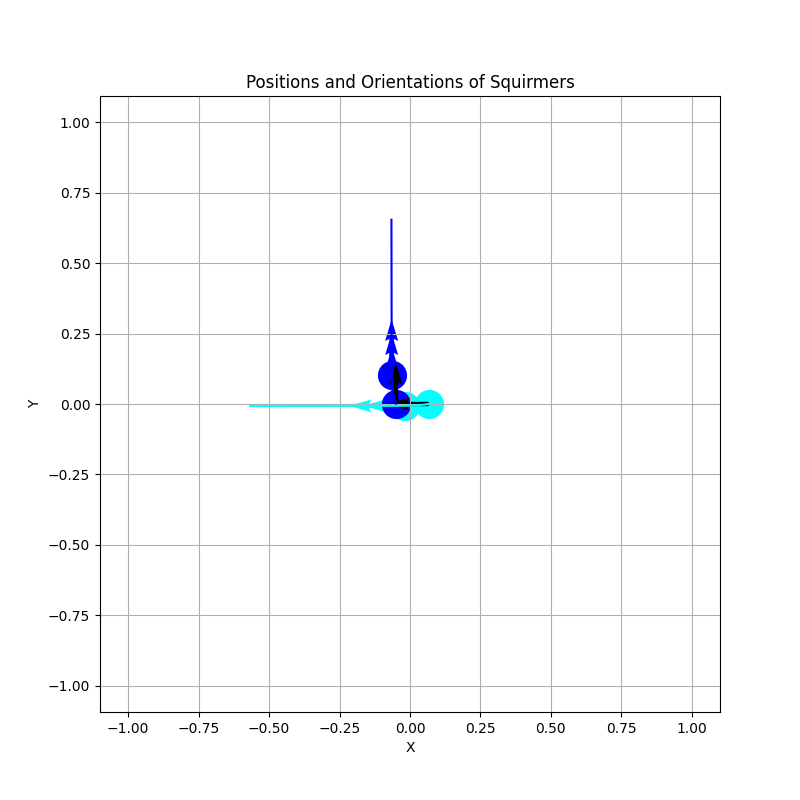
\includegraphics[width=1\textwidth]{graphs/Eo_analysis/beta0/pi_/pi_Eo_brumley.png}
        \caption{\footnotesize Simulation parameters: $a=0.05$, $v_0=1$, $\beta_1=0$, $\mu=1$ and $E_{0_{2}}=\frac{8}{5}\mu\pi a^2$}
    \end{minipage}\hfill
    \begin{minipage}{0.49\textwidth}
        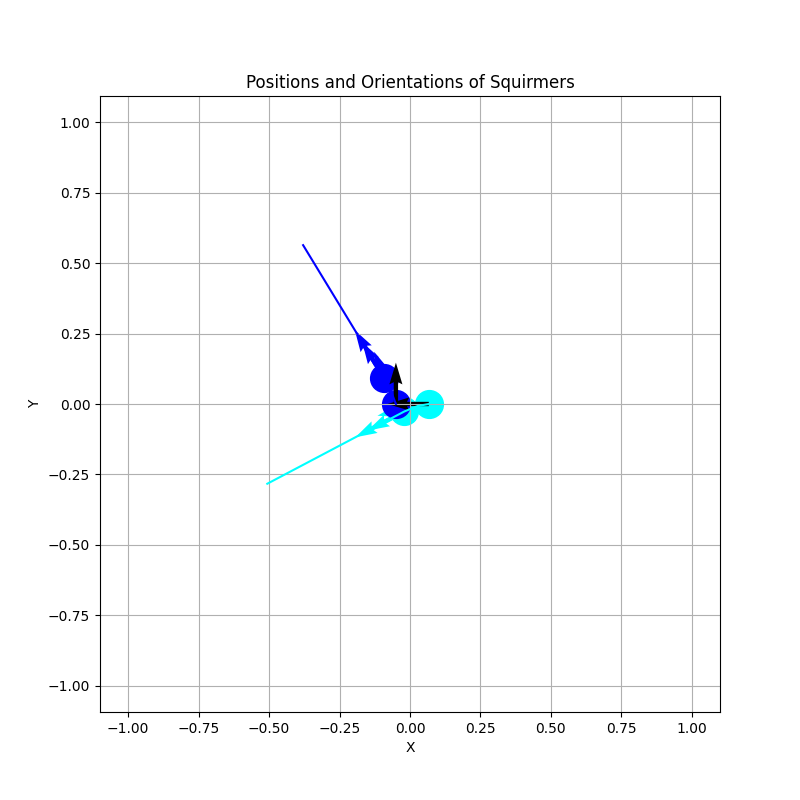
\includegraphics[width=1\textwidth]{graphs/Eo_analysis/beta0/pi_/pi_Eo_init.png}
        \caption{\footnotesize Simulation parameters: $a=0.05$, $v_0=1$, $\beta_1=0$, $\mu=1$ and $E_{0_{1}}=\frac{3}{10}\frac{v_0}{a}$}
    \end{minipage}
    \begin{minipage}{0.49\textwidth}
        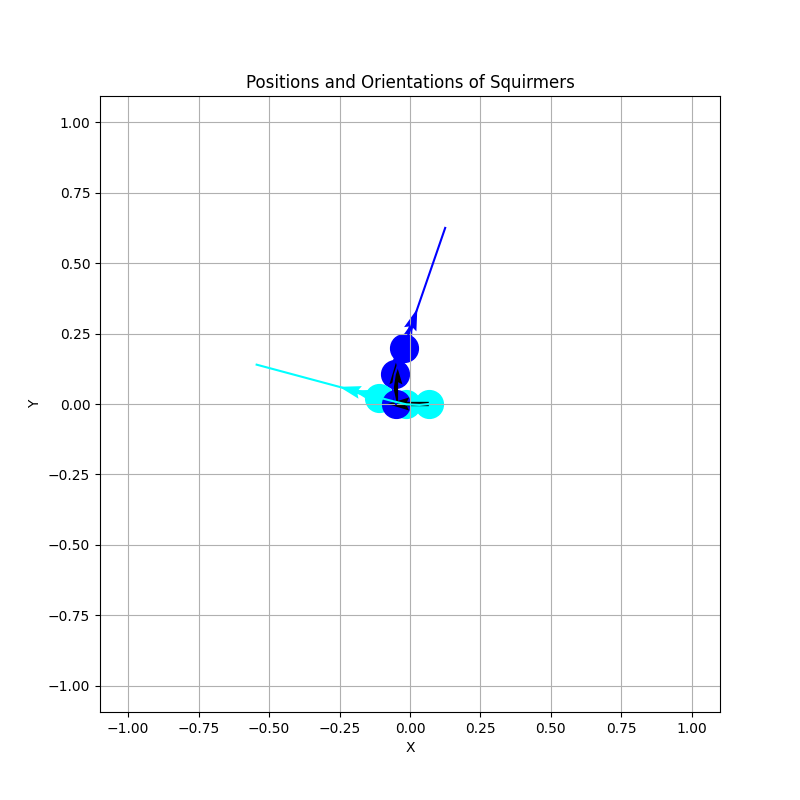
\includegraphics[width=1\textwidth]{graphs/Eo_analysis/beta0/pi_/pi_m2.png}
        \caption{\footnotesize Simulation parameters: $a=0.05$, $v_0=1$, $\beta_1=0$, $\mu=1$ and $E_{0_{7}}=-2$}
    \end{minipage}\hfill
    \begin{minipage}{0.49\textwidth}
        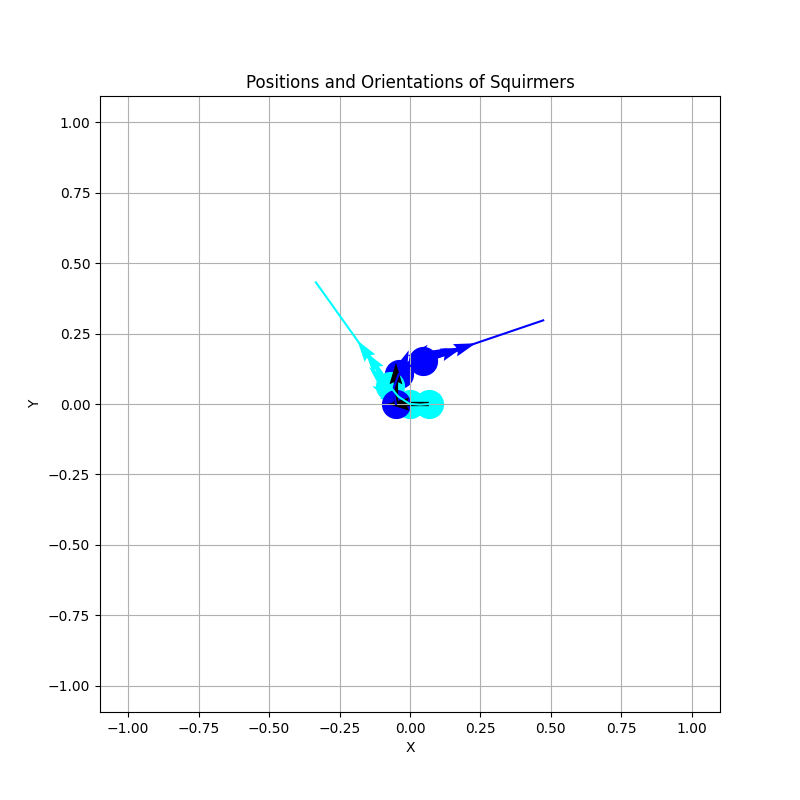
\includegraphics[width=1\textwidth]{graphs/Eo_analysis/beta0/pi_/pi_m5.png}
        \caption{\footnotesize Simulation parameters: $a=0.05$, $v_0=1$, $\beta_1=0$, $\mu=1$ and $E_{0_{5}}=-5$}
    \end{minipage}
    position and orientation of squirmer1: $(x1,y1)=(-a,0)$, $\theta_1=\frac{\pi}{2}$\\
    position and orientation of squirmer2: $(x2,y2)=(\frac{2a}{1.5},0)$, $\theta_2=\pi$\\
    The arrows shows when the orientations of the squirmers are affected and a circle is plotted every four time the orientation of a squirmer is affected
\end{figure}

\subsection{N squirmers}
The first step was to modify the code done during the initial project to simulate the behavior of $N$ squirmers.

\newpage

\nocite{*}
\bibliographystyle{plain}
\bibliography{bibliography/biblio}
\end{document}